% CuentaConmigo · presentación del proyecto (versión preliminar para corrección del autor)
% Compilar: pdflatex cuentaconmigo.tex (dos veces). Ver README.md.
% Sólo paquetes estándar de TeX Live: beamer, tikz, xcolor, babel (spanish), pifont, amssymb.
\documentclass[aspectratio=169,11pt]{beamer}

\usepackage[utf8]{inputenc}
\usepackage[T1]{fontenc}
\usepackage{lmodern}
\usepackage[spanish,es-noshorthands,es-tabla]{babel}
\usepackage{xcolor}
\usepackage{tikz}
\usetikzlibrary{positioning,calc,arrows.meta,shapes.misc}
\usepackage{graphicx}
\usepackage{etoolbox}
\usepackage{pifont}
\usepackage{amssymb}
\usepackage{textcomp}
\graphicspath{{../cover/}}

% ---------------------------------------------------------------------------
% Paleta: tomada de design/prototypes (tema claro) y design/cover/cover.png
% ---------------------------------------------------------------------------
\definecolor{ccblue}{HTML}{1D4F91}   % acento (tema claro)
\definecolor{ccsky}{HTML}{7CB9E8}    % acento (tema oscuro / portada)
\definecolor{ccnavy}{HTML}{0E1524}   % fondo oscuro
\definecolor{ccamber}{HTML}{F6B40E}  % foco / aviso / marca
\definecolor{ccbg}{HTML}{EEF2F7}     % fondo claro
\definecolor{ccfg}{HTML}{14213A}     % texto
\definecolor{ccmuted}{HTML}{5B6B86}  % texto secundario
\definecolor{ccborder}{HTML}{C8D2E2}
\definecolor{ccok}{HTML}{2E7D52}
\definecolor{ccokbg}{HTML}{DDF5E6}
\definecolor{ccerr}{HTML}{C0392B}
\definecolor{ccerrbg}{HTML}{FBE3E0}
\definecolor{ccwarnbg}{HTML}{FFF1C2}
\definecolor{ccwarnfg}{HTML}{5C4300}

% ---------------------------------------------------------------------------
% Tema Beamer (mínimo, sobre el tema default)
% ---------------------------------------------------------------------------
\setbeamertemplate{navigation symbols}{}
\setbeamercolor{normal text}{fg=ccfg,bg=white}
\setbeamercolor{structure}{fg=ccblue}
\setbeamercolor{frametitle}{fg=ccblue,bg=white}
\setbeamerfont{frametitle}{series=\bfseries,size=\Large}
\setbeamercolor{block title}{fg=white,bg=ccblue}
\setbeamercolor{block body}{fg=ccfg,bg=ccbg}
\setbeamercolor{block title alerted}{fg=ccnavy,bg=ccamber}
\setbeamercolor{block body alerted}{fg=ccfg,bg=ccwarnbg}
\setbeamercolor{block title example}{fg=white,bg=ccok}
\setbeamercolor{block body example}{fg=ccfg,bg=ccokbg}
\setbeamertemplate{blocks}[rounded]
\setbeamertemplate{itemize items}[circle]
\setbeamercolor{itemize item}{fg=ccblue}
\setbeamercolor{itemize subitem}{fg=ccsky}
\setbeamertemplate{frametitle}{%
  \vspace{6pt}%
  {\usebeamerfont{frametitle}\usebeamercolor[fg]{frametitle}\insertframetitle\par}%
  \vspace{1pt}{\color{ccamber}\rule{18pt}{2pt}}\par\vspace{2pt}%
}
\setbeamertemplate{footline}{%
  \begin{beamercolorbox}[wd=\paperwidth,ht=2.4ex,dp=1ex,leftskip=10mm,rightskip=10mm]{normal text}%
    \usebeamerfont{footline}\scriptsize\color{ccmuted}%
    CuentaConmigo \textperiodcentered\ versión preliminar \textperiodcentered\ 31/10/2026%
    \hfill github.com/kenarab/cuentaconmigo \textperiodcentered\ \insertframenumber/\inserttotalframenumber
  \end{beamercolorbox}%
}
\hypersetup{colorlinks=true,urlcolor=ccblue,linkcolor=ccblue}

% ---------------------------------------------------------------------------
% Maquetas de teléfono (TikZ) y elementos de UI
% ---------------------------------------------------------------------------
% \phonemock[rótulo]{ancho}{alto}{contenido}
\newlength{\phonetop}
\newcommand{\phonemock}[4][]{%
  \begin{tikzpicture}[baseline=(body.south)]
    \ifstrempty{#1}{\setlength{\phonetop}{8pt}}{\setlength{\phonetop}{20pt}}%
    \node[draw=ccnavy,fill=ccnavy,line width=1.2pt,rounded corners=10pt,inner sep=0pt,
          minimum width=#2,minimum height=#3] (body) {};
    \node[fill=white,rounded corners=6pt,inner sep=5pt,anchor=north,align=left,font=\tiny,
          text width=\dimexpr#2-16pt-10pt\relax,
          minimum height=\dimexpr#3-\phonetop-8pt\relax]
          (screen) at ([yshift=-\phonetop]body.north)
          {\setlength{\fboxsep}{1.5pt}\setlength{\fboxrule}{0.4pt}#4};
    \ifstrempty{#1}{%
      \fill[ccnavy!50!white] ([yshift=-4pt]body.north) circle (1.2pt);
    }{%
      \node[fill=ccamber,text=ccnavy,font=\tiny\bfseries,inner sep=2pt,anchor=north,
            minimum width=\dimexpr#2-16pt\relax] at ([yshift=-4pt]body.north) {#1};
    }%
  \end{tikzpicture}%
}
\newcommand{\uibar}[2]{\makebox[\linewidth][s]{\textcolor{ccmuted}{#1}\hfill\textcolor{ccmuted}{#2}}\\[2pt]}
\newcommand{\uititle}[1]{{\scriptsize\bfseries #1}\\[2pt]}
\newcommand{\uisec}[1]{\textcolor{ccmuted}{\textsc{#1}}\\[1pt]}
\newcommand{\uirow}[2]{\makebox[\linewidth][s]{#1\hfill\fcolorbox{ccborder}{ccbg}{\texttt{#2}}}\\[1.5pt]}
\newcommand{\uidrop}[2]{\textcolor{ccmuted}{#1}\\[0.5pt]\fcolorbox{ccborder}{white}{\makebox[\dimexpr\linewidth-2\fboxsep-2\fboxrule\relax][s]{#2\hfill\textcolor{ccblue}{$\blacktriangledown$}}}\\[2pt]}
\newcommand{\uibtn}[1]{\colorbox{ccblue}{\makebox[\dimexpr\linewidth-2\fboxsep\relax][c]{\textcolor{white}{\bfseries #1}}}\\[2pt]}
\newcommand{\uibtns}[1]{\fcolorbox{ccblue}{white}{\makebox[\dimexpr\linewidth-2\fboxsep-2\fboxrule\relax][c]{\textcolor{ccblue}{#1}}}\\[2pt]}
\newcommand{\uichip}[1]{\fcolorbox{ccblue}{ccsky!25!white}{\texttt{#1}}}
\newcommand{\uiimg}[2]{\colorbox{ccbg}{\makebox[\dimexpr\linewidth-2\fboxsep\relax][c]{\rule{0pt}{#1}\textcolor{ccmuted}{#2}}}\\[2pt]}
\newcommand{\uiwarn}[1]{\colorbox{ccwarnbg}{\parbox{\dimexpr\linewidth-2\fboxsep\relax}{\textcolor{ccwarnfg}{\textbf{!}\ #1}}}\\[2pt]}
\newcommand{\uiok}[1]{\colorbox{ccokbg}{\parbox{\dimexpr\linewidth-2\fboxsep\relax}{\textcolor{ccok}{\ding{51}\ #1}}}\\[2pt]}
\newcommand{\uierr}[1]{\colorbox{ccerrbg}{\parbox{\dimexpr\linewidth-2\fboxsep\relax}{\textcolor{ccerr}{\ding{55}\ #1}}}\\[2pt]}
\newcommand{\uinote}[1]{\textcolor{ccmuted}{\emph{#1}}\\[1pt]}
\newcommand{\uistatus}[2]{\makebox[\linewidth][s]{#1\hfill\textcolor{#2}{\ding{108}}}\\[1pt]}

% Tarjeta de principio (TikZ)
\tikzset{
  card/.style={draw=ccborder,fill=ccbg,rounded corners=4pt,inner sep=6pt,text width=#1,align=left,font=\footnotesize},
  cardtitle/.style={font=\footnotesize\bfseries,text=ccblue},
  box/.style={draw=ccblue,fill=white,rounded corners=3pt,inner sep=4pt,align=center,font=\scriptsize,text width=#1},
  boxdark/.style={draw=ccnavy,fill=ccnavy,text=white,rounded corners=3pt,inner sep=4pt,align=center,font=\scriptsize,text width=#1},
  boxamber/.style={draw=ccamber,fill=ccwarnbg,rounded corners=3pt,inner sep=4pt,align=center,font=\scriptsize,text width=#1},
  flow/.style={-{Stealth[length=5pt]},ccblue,thick},
  flowd/.style={-{Stealth[length=5pt]},ccmuted,thick,dashed},
}

\title{CuentaConmigo}
\author{Proyecto abierto \textperiodcentered\ github.com/kenarab/cuentaconmigo}
\date{31 de octubre de 2026}

\begin{document}

% ===========================================================================
% 1 · Portada
% ===========================================================================
\begin{frame}[plain]
  \begin{tikzpicture}[remember picture,overlay]
    \shade[top color=ccblue,bottom color=ccsky!70!ccblue] (current page.south west) rectangle (current page.north east);
    % red de puntos decorativa (sin datos)
    \foreach \x/\y in {0.8/1.1, 2.4/0.6, 4.1/1.4, 6.0/0.5, 8.3/1.2, 10.5/0.7, 12.6/1.5, 14.4/0.9}{
      \fill[white,opacity=0.55] ($(current page.south west)+(\x cm,\y cm)$) circle (2pt);
    }
    \draw[white,opacity=0.35,thick]
      ($(current page.south west)+(0.8cm,1.1cm)$) -- ($(current page.south west)+(2.4cm,0.6cm)$) --
      ($(current page.south west)+(4.1cm,1.4cm)$) -- ($(current page.south west)+(6.0cm,0.5cm)$) --
      ($(current page.south west)+(8.3cm,1.2cm)$) -- ($(current page.south west)+(10.5cm,0.7cm)$) --
      ($(current page.south west)+(12.6cm,1.5cm)$) -- ($(current page.south west)+(14.4cm,0.9cm)$);
  \end{tikzpicture}
  \vspace*{2mm}
  \begin{center}
    \IfFileExists{../cover/cover.png}{%
      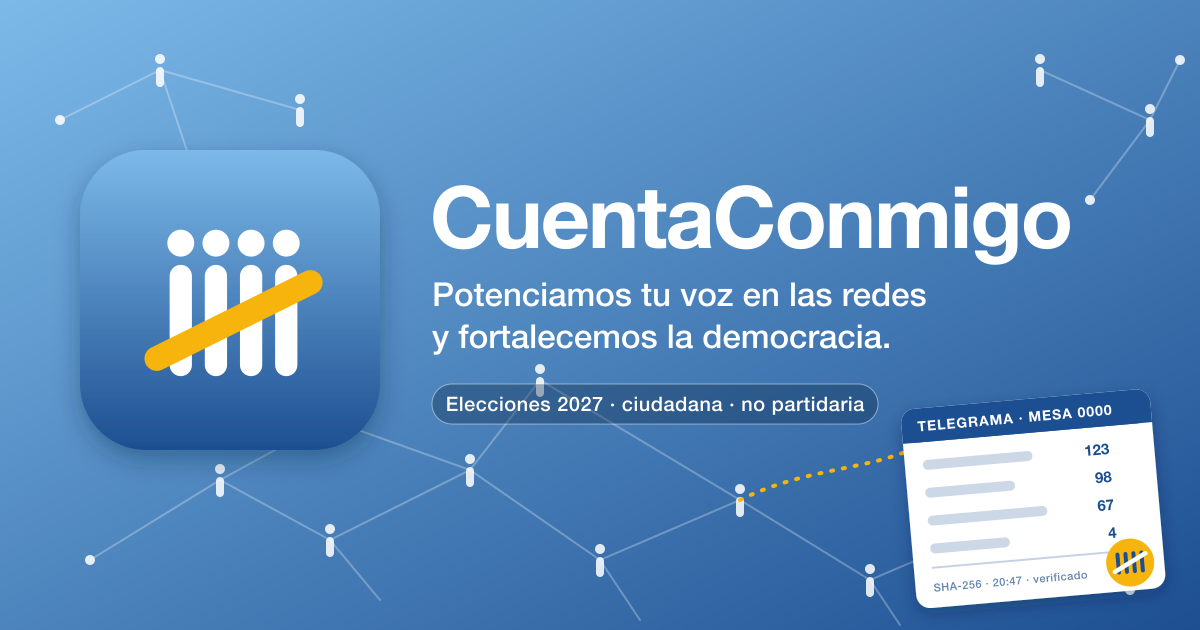
\includegraphics[width=0.72\paperwidth]{cover.png}%
    }{%
      \begin{tikzpicture}
        \node[fill=white,rounded corners=10pt,minimum width=0.78\paperwidth,minimum height=38mm,align=center] {%
          {\Huge\bfseries\color{ccblue}CuentaConmigo}\\[4pt]
          {\large\color{ccfg}Potenciamos tu voz en las redes y fortalecemos la democracia.}\\[4pt]
          {\small\color{ccmuted}Elecciones 2027 \textperiodcentered\ ciudadana \textperiodcentered\ no partidaria}};
      \end{tikzpicture}%
    }
  \end{center}
  \vspace{1mm}
  \begin{center}
    \color{white}
    {\small Red social ciudadana y no partidaria para cuidar el proceso democrático de las elecciones argentinas de 2027.}\\[3pt]
    {\footnotesize Presentación del proyecto \textperiodcentered\ \textbf{versión preliminar} para corrección del autor \textperiodcentered\ 31/10/2026}\\[2pt]
    {\footnotesize Código y especificaciones abiertos: \textbf{github.com/kenarab/cuentaconmigo}}
  \end{center}
\end{frame}

% ===========================================================================
% 2 · Problema
% ===========================================================================
\begin{frame}{El problema: la conversación electoral corre con reglas ajenas}
  \begin{columns}[T]
    \begin{column}{0.56\textwidth}
      \begin{itemize}
        \item Millones de personas opinamos y nos organizamos en redes de grandes empresas.
              Sus algoritmos deciden qué se ve, a quién se vende publicidad y qué pasa con la desinformación.
        \item La única vía ciudadana es el botón de denuncia de cada plataforma: sin saber qué pasa después
              y sin medición pública de lo que hacen.
        \item El dinero electoral puede financiar desinformación viral. Nadie lo mide de forma independiente
              y reproducible.
        \item El cierre del proceso, el escrutinio de mesa, depende de fiscales que anotan a mano,
              de noche, bajo presión y sin herramientas comunes.
      \end{itemize}
      \vspace{2pt}
      \begin{alertblock}{Lo que falta}
        Un espacio propio para \textbf{medir desde afuera}, \textbf{deliberar} y \textbf{decidir juntos} qué hacer,
        con reglas iguales para todas las fuerzas.
      \end{alertblock}
    \end{column}
    \begin{column}{0.42\textwidth}
      \centering
      \begin{tikzpicture}[node distance=5pt]
        \node[boxdark=118pt,minimum height=50pt] (plat) {\textbf{Plataformas}\\[2pt]
          {\tiny algoritmo \textperiodcentered\ publicidad \textperiodcentered\ moderación}\\[2pt]
          \colorbox{ccnavy!70!white}{\textcolor{white}{\tiny conversación electoral de millones}}};
        \node[box=118pt,below=14pt of plat] (ciu) {\textbf{Ciudadanía}\\{\tiny opina, discute, se organiza}};
        \draw[flowd] (ciu.north) -- node[right,font=\tiny,text=ccmuted,align=left]{botón de denuncia\\sin respuesta} (plat.south);
        \node[boxamber=118pt,below=12pt of ciu] (cc) {\textbf{CuentaConmigo}\\{\tiny mide \textperiodcentered\ delibera \textperiodcentered\ decide por consenso}};
        \draw[flow] (ciu.south) -- (cc.north);
        \draw[flow] (cc.west) -- ++(-10pt,0) |- node[pos=0.25,left,font=\tiny,text=ccblue,align=right]{medición\\pública} (plat.west);
      \end{tikzpicture}
    \end{column}
  \end{columns}
\end{frame}

% ===========================================================================
% 3 · Qué es la red
% ===========================================================================
\begin{frame}{Qué es CuentaConmigo: una red para cuidar las reglas de juego}
  \begin{center}
  \begin{tikzpicture}[node distance=5pt]
    \node[card=80pt] (p1) {\textcolor{ccblue}{\bfseries No partidaria}\\[2pt]
      Cuida el proceso, no compite en él. No hace campaña ni promueve candidaturas.};
    \node[card=80pt,right=of p1] (p2) {\textcolor{ccblue}{\bfseries Todos los partidos, en igualdad}\\[2pt]
      Mismas herramientas, reglas y visibilidad para todas las fuerzas.};
    \node[card=80pt,right=of p2] (p3) {\textcolor{ccblue}{\bfseries Consenso antes que acción}\\[2pt]
      Ninguna acción externa sin consenso registrado y chequeo legal electoral.};
    \node[card=80pt,right=of p3] (p4) {\textcolor{ccblue}{\bfseries La UX es fundamental}\\[2pt]
      Quien fiscaliza lo hace bajo presión: se elige, no se tipea; mínimos pasos.};
  \end{tikzpicture}
  \end{center}
  \vspace{2pt}
  {\footnotesize También: evidencia verificable (hash y fecha), herramientas propias (no los botones de denuncia),
  sin amplificación paga, código y datos agregados abiertos, privacidad primero (la afinidad política es un dato sensible y no se pide).}
  \vspace{4pt}
  \begin{center}
  \begin{tikzpicture}[node distance=5pt]
    \node[box=64pt] (a) {\textbf{A \textperiodcentered\ Plataformas}\\publicidad, algoritmos, veda, compromisos};
    \node[box=64pt,right=of a] (b) {\textbf{B \textperiodcentered\ Desinformación}\\detección, verificación, respuesta};
    \node[box=64pt,right=of b] (c) {\textbf{C \textperiodcentered\ Campaña}\\gasto declarado vs.\ observado};
    \node[box=64pt,right=of c,draw=ccamber,fill=ccwarnbg] (d) {\textbf{D \textperiodcentered\ Jornada y escrutinio}\\telegramas, actas, cotejo};
    \node[box=64pt,right=of d] (e) {\textbf{E \textperiodcentered\ Propuestas}\\deliberación e incidencia};
    \node[font=\scriptsize\bfseries,text=ccmuted,above=4pt of c] {Herramientas que la red activa por consenso};
    \node[font=\tiny,text=ccmuted,below=3pt of c] {D cierra la auditoría ciudadana; hoy es la parte que funciona (app y simulación).};
  \end{tikzpicture}
  \end{center}
\end{frame}

% ===========================================================================
% 4 · App de escrutinio hoy
% ===========================================================================
\begin{frame}{La app de escrutinio, hoy (prototipo iOS)}
  \begin{center}
  \phonemock{122pt}{172pt}{%
    \uibar{$\leftarrow$ Certificado}{Paso 2/4}
    \uititle{Datos de la mesa}
    \uidrop{Distrito}{Buenos Aires}
    \uidrop{Sección}{Tercera}
    \uidrop{Establecimiento (buscar)}{Escuela N.\textordmasculine\ 12 (ejemplo)}
    \uidrop{Mesa}{0421}
    \uinote{Elegís, no tipeás. Al elegir la mesa se completa el resto.}
    \uibtns{Usar un telegrama de ejemplo}
    \uibtn{Continuar}
  }\hfill
  \phonemock{122pt}{172pt}{%
    \uibar{$\leftarrow$ Mesa 0421}{Paso 4/4}
    \uiimg{20pt}{imagen pág.\ 1/2 \textperiodcentered\ ampliar}
    \uisec{Totales de la mesa}
    \uirow{Electores}{350}
    \uirow{Total de votantes}{225}
    \uisec{Presidente y Vice}
    \uirow{Lista A (ficticia)}{123}
    \uirow{Lista B (ficticia)}{\textcolor{ccblue}{$\mid$}\ \ }
    \uirow{Lista C (ficticia)}{\ \ \ }
    \uinote{Detectados por OCR: tocá para copiar}
    \uichip{98}\ \uichip{4}\ \uichip{225}\ \uichip{0}\\[2pt]
    \uiwarn{La suma no coincide con votantes}
    \uibtn{Validar}
  }\hfill
  \phonemock{122pt}{172pt}{%
    \uibar{$\leftarrow$ Validación}{Paso 4/4}
    \uititle{Confirmar captura}
    Mesa 0421 \textperiodcentered\ Certificado\\
    2 páginas \textperiodcentered\ 16 valores\\[2pt]
    \uiwarn{1 aviso con justificación: ``El acta dice 223.''}
    \uisec{Evidencia}
    SHA-256 \texttt{3f9c\ldots a1e2}\\
    Fecha UTC \texttt{AAAA-MM-DD 21:47}\\[2pt]
    \uinote{Al confirmar, la captura queda bloqueada: no se edita ni se borra. Si hay un error, hacé una nueva captura.}
    \uibtn{Confirmar y bloquear}
    \uibtns{Volver a revisar}
  }
  \end{center}
  \vspace{2pt}
  {\scriptsize\color{ccmuted} Flujo guiado: aviso de Boleta Única $\to$ tipo de documento $\to$ mesa $\to$ escaneo $\to$ carga $\to$ validación $\to$ bloqueo.
  Plantilla ficticia: ``Lista A/B/C'' son rótulos de demo, no fuerzas reales. El OCR sugiere, nunca completa solo; cada valor viaja con su origen.}
\end{frame}

% ===========================================================================
% 5 · Tres diseños F-1 / F-2 / F-3
% ===========================================================================
\begin{frame}{Tres diseños sobre el mismo flujo: F-1, F-2 y F-3}
  \begin{columns}[T]
    \begin{column}{0.33\textwidth}
      \centering
      \phonemock{104pt}{112pt}{%
        \uibar{$\leftarrow$ Paso 5 de 7}{}
        \uititle{Presidente y Vice (1/2)}
        \uirow{Lista A (ficticia)}{123}
        \uirow{Lista B (ficticia)}{98}
        \uirow{En blanco}{4}
        \uibtn{Siguiente categoría}
      }\\[2pt]
      {\footnotesize\textbf{F-1 \textperiodcentered\ Asistente paso a paso}}\\
      {\scriptsize Una pregunta por pantalla. Imposible saltear el aviso legal; muchos toques bajo presión.}
    \end{column}
    \begin{column}{0.33\textwidth}
      \centering
      \phonemock{104pt}{112pt}{%
        \uibar{$\leftarrow$ Mesa 0421}{Acta $\blacktriangledown$}
        \uiimg{14pt}{imagen fija \textperiodcentered\ zoom}
        \uirow{Lista A (ficticia)}{123}
        \uirow{Lista B (ficticia)}{\textcolor{ccblue}{$\mid$}\ \ }
        \uichip{98}\ \uichip{4}\ \uichip{225}\\[1pt]
        \textcolor{ccmuted}{\texttt{1 2 3 \ \ 4 5 6 \ \ 7 8 9}}
      }\\[2pt]
      {\footnotesize\textbf{F-2 \textperiodcentered\ Vista partida}}\\
      {\scriptsize Imagen arriba, campos abajo, fichas del OCR sobre el teclado. Menos toques; todo a la vista.}
    \end{column}
    \begin{column}{0.33\textwidth}
      \centering
      \phonemock{104pt}{112pt}{%
        \uititle{Comparación}
        \uiok{Coinciden 11 de 14 valores}
        Presidente \textperiodcentered\ Lista B\\
        carga 1: \uichip{98}\ \ carga 2: \uichip{89}\\[1pt]
        Diputados \textperiodcentered\ En blanco\\
        carga 1: \uichip{4}\ \ carga 2: \uichip{14}\\[1pt]
        \uibtns{Ver imagen y resolver}
      }\\[2pt]
      {\footnotesize\textbf{F-3 \textperiodcentered\ Doble carga a ciegas}}\\
      {\scriptsize Dos personas cargan sin verse; la app sólo pide resolver diferencias. Sin registrar quién fue cada una.}
    \end{column}
  \end{columns}
  \vspace{4pt}
  \begin{block}{Decisión de diseño (consenso \#2, aceptado por el autor)}
    \footnotesize Los tres diseños conviven en la app y se eligen desde ``Acerca de'' para compararlos en campo.
    Recomendación: híbrido F-1 (preparación en cuatro pasos) + F-2 (carga en una pantalla), con F-3 como verificación opcional.
  \end{block}
\end{frame}

% ===========================================================================
% 6 · Simulación AMBA
% ===========================================================================
\begin{frame}{Simulación del AMBA: por qué cada carga suma}
  \begin{columns}[T]
    \begin{column}{0.5\textwidth}
      \centering
      {\footnotesize\textbf{Error máximo (mediana de 30 semillas, puntos porcentuales)}}\\[2pt]
      \begin{tikzpicture}[x=1pt,y=1pt]
        % leyenda
        \fill[ccamber] (0,106) rectangle ++(8,6); \node[font=\tiny,right] at (8,109) {suma ingenua de las mesas cargadas};
        \fill[ccblue] (0,96) rectangle ++(8,6); \node[font=\tiny,right] at (8,99) {estimación estratificada por electores};
        % ejes y grilla
        \foreach \v in {1,2,3,4}{
          \draw[ccborder] (0,\v*22) -- (190,\v*22);
          \node[font=\tiny,text=ccmuted,left=1pt] at (0,\v*22) {\v};
        }
        \draw[ccmuted] (0,0) -- (190,0);
        \draw[ccmuted] (0,0) -- (0,92);
        % escenarios: x / ingenua / estratificada / rótulo ingenua / rótulo estratificada / escenario
        \foreach \px/\ing/\est/\ingt/\estt/\lab in {%
          20/0.28/0.24/{0,28}/{0,24}/{sesgo 0 \textperiodcentered\ 5\,\%},%
          65/3.08/0.22/{3,08}/{0,22}/{sesgo 0,7 \textperiodcentered\ 5\,\%},%
          110/3.93/0.18/{3,93}/{0,18}/{sesgo 1 \textperiodcentered\ 5\,\%},%
          155/4.00/0.35/{4,00}/{0,35}/{sesgo 1 \textperiodcentered\ 2\,\%}}{
          \fill[ccamber] (\px,0) rectangle ++(14,\ing*22);
          \fill[ccblue] (\px+16,0) rectangle ++(14,\est*22);
          \node[font=\tiny,above,text=ccwarnfg] at (\px+7,\ing*22) {\ingt};
          \node[font=\tiny,above,text=ccblue] at (\px+23,\est*22) {\estt};
          \node[font=\tiny,below,text=ccmuted] at (\px+15,-1) {\lab};
        }
      \end{tikzpicture}\\[4pt]
      {\tiny\color{ccmuted} Puntos porcentuales sobre votos afirmativos. Mediciones de \texttt{sdd/specs/amba-simulation}, 31/10/2026.}
    \end{column}
    \begin{column}{0.48\textwidth}
      \footnotesize
      \begin{itemize}
        \item \textbf{Datos reales:} escrutinio provisorio de las generales del 22/10/2023 (DINE), Presidente y Vice.
              29\,962 mesas, 39 estratos (15 comunas + 24 partidos), 10\,413\,971 electores. Procedencia con URL, fecha y SHA-256.
        \item \textbf{Modelo:} estimador de razón estratificado por electores, con intervalo del 95\,\%.
        \item \textbf{Con sesgo de llegada} (CABA reporta antes que el conurbano) la suma ingenua se desvía 3--4 puntos;
              la estratificada queda por debajo de 0,4 con el 5\,\% de las mesas.
        \item \textbf{Cobertura del intervalo del 95\,\%:} entre 92,5\,\% y 96,0\,\% según el escenario (40 semillas $\times$ 5 listas).
        \item Las fuerzas se muestran como Lista A--E; el mapeo real queda en los datos, fuera de pantalla.
      \end{itemize}
      \begin{alertblock}{SIMULACIÓN \textperiodcentered\ reproducción de las generales 2023}
        \scriptsize El art.\ 71 inc.\ h del Código Electoral prohíbe publicar proyecciones durante una elección en curso y hasta tres horas después del cierre. Esta reproducción no es una proyección.
      \end{alertblock}
    \end{column}
  \end{columns}
\end{frame}

% ===========================================================================
% 7 · Backend y OCR
% ===========================================================================
\begin{frame}{Backend y OCR: dos escrutinios, un cotejo (propuesta)}
  \begin{columns}[T]
    \begin{column}{0.58\textwidth}
      \centering
      \begin{tikzpicture}[node distance=7pt and 8pt]
        \node[box=52pt] (app) {\textbf{App}\\captura con hash};
        \node[box=58pt,right=of app] (api) {\textbf{API de ingesta}\\valida, recomputa hash, idempotente};
        \node[box=58pt,right=of api] (store) {\textbf{Blobs + DB}\\inmutables, con procedencia};
        \node[box=58pt,below=of api] (ocr) {\textbf{Workers OCR}\\Tesseract hoy; dígitos por región después};
        \node[box=58pt,below=of store] (rev) {\textbf{Revisión humana}\\doble carga a ciegas};
        \node[box=58pt,below=of ocr] (agg) {\textbf{Agregador}\\estratificado + IC};
        \node[boxdark=58pt,below=of rev] (mirror) {\textbf{Espejo oficial}\\DINE / CNE, versionado};
        \node[boxamber=52pt,left=of agg] (qc) {\textbf{Conteo rápido}\\muestra sorteada\\embargo art.\ 71 h};
        \node[box=58pt,below=of agg] (cmp) {\textbf{Cotejo mesa a mesa}\\``diferencia'', nunca ``fraude''};
        \draw[flow] (app) -- (api);
        \draw[flow] (api) -- (store);
        \draw[flow] (api) -- (ocr);
        \draw[flow] (store) -- (rev);
        \draw[flowd] (ocr) -- node[above,font=\tiny,text=ccmuted]{sugiere} (rev);
        \draw[flow] (rev) -- (agg);
        \draw[flow] (agg) -- (qc);
        \draw[flow] (agg) -- (cmp);
        \draw[flow] (mirror) |- (cmp);
      \end{tikzpicture}
    \end{column}
    \begin{column}{0.4\textwidth}
      \footnotesize
      \begin{itemize}
        \item \textbf{Regla:} lo extraído por OCR nunca se mezcla con lo confirmado por personas. Sólo los valores confirmados cuentan.
        \item \textbf{Medición de base (provisoria):} Tesseract 5 sobre 14 muestras encuentra el \textbf{72,4\,\%} (399/551) de los valores transcriptos entre los números de la página. No mide la posición: falta la extracción por regiones y la métrica por celda.
        \item \textbf{Embargo:} el conteo rápido se calcula desde la primera carga y \textbf{no se publica} hasta que vence la ventana del art.\ 71 inc.\ h (cierre + 3 h, a verificar). Acceso con registro mientras dura.
        \item \textbf{Sin datos personales:} dispositivos con identidad seudónima; imágenes con acceso restringido y retención limitada.
        \item Stack propuesto: Python para el prototipo, camino a Rust; API REST \texttt{/v1}. Nada se instala sin el autor.
      \end{itemize}
    \end{column}
  \end{columns}
\end{frame}

% ===========================================================================
% 8 · Funcionalidades que todavía no hacemos
% ===========================================================================
\begin{frame}{Lo que todavía no hacemos: maquetas de lo que viene}
  \begin{center}
  \phonemock[PRÓXIMAMENTE \textperiodcentered\ maqueta]{94pt}{162pt}{%
    \uititle{Mi plan del día}
    \uinote{Escuela N.\textordmasculine\ 12 (ejemplo)}
    \uistatus{Mesa 0418 \textperiodcentered\ cotejada}{ccok}
    \uistatus{Mesa 0419 \textperiodcentered\ capturada}{ccok}
    \uistatus{Mesa 0420 \textperiodcentered\ visitada}{ccamber}
    \uistatus{Mesa 0421 \textperiodcentered\ pendiente}{ccmuted}
    \uistatus{Mesa 0422 \textperiodcentered\ incidencia}{ccerr}
    \uiok{0421: captura de otra persona. Coincide celda a celda.}
    \uinote{Te faltan 2 mesas sin captura. Cierre: 18:00.}
    \uibtn{Capturar 0421}
  }\hfill
  \phonemock[PRÓXIMAMENTE \textperiodcentered\ maqueta]{94pt}{162pt}{%
    \uititle{Invitar en persona}
    \begin{tikzpicture}[x=2.2pt,y=2.2pt]
      \foreach \i in {0,...,13}{\foreach \j in {0,...,13}{
        \pgfmathtruncatemacro{\qrv}{mod(\i*7+\j*3+int(\i/3),4)}
        \ifnum\qrv<2 \fill[ccnavy] (\i,\j) rectangle ++(1,1);\fi
      }}
      \fill[white] (0,0) rectangle (4,4); \draw[ccnavy,line width=1.2pt] (0.5,0.5) rectangle (3.5,3.5);
      \fill[white] (10,0) rectangle (14,4); \draw[ccnavy,line width=1.2pt] (10.5,0.5) rectangle (13.5,3.5);
      \fill[white] (0,10) rectangle (4,14); \draw[ccnavy,line width=1.2pt] (0.5,10.5) rectangle (3.5,13.5);
    \end{tikzpicture}\\[1pt]
    \uinote{QR de un solo uso. Quien entra queda en tu rama; no se guardan nombres ni DNI.}
    \uirow{Tu nivel}{2}
    \uirow{Cupo del mes}{3 de 5}
    \uibtn{Generar QR}
  }\hfill
  \phonemock[PRÓXIMAMENTE \textperiodcentered\ maqueta]{94pt}{162pt}{%
    \uititle{Dictamen del panel}
    \uinote{Carta abierta sobre anuncios en veda (ejemplo ilustrativo)}
    \uirow{Panel sorteado}{9}
    \uirow{Evidencia con hash}{\ding{51}}
    \uirow{Neutralidad (0--3)}{3}
    \uirow{Proporcionalidad}{2}
    \uirow{Métrica previa}{\ding{51}}
    \uiok{Adoptar con cambios \textperiodcentered\ 2 disidencias}
    \uinote{Sigue: ratificación y chequeo legal.}
    \uibtns{Leer expediente}
  }\hfill
  \phonemock[PRÓXIMAMENTE \textperiodcentered\ maqueta]{94pt}{162pt}{%
    \uititle{Conteo rápido propio}
    \uinote{Muestra: 1\,200 mesas sorteadas \textperiodcentered\ 48\,\% confirmadas}
    \uinote{Ejemplo ilustrativo, no es un resultado. Listas ficticias.}
    \uirow{Lista A (fict.)}{38,4 $\pm$ 1,2}
    \uirow{Lista B (fict.)}{31,9 $\pm$ 1,1}
    \uirow{Lista C (fict.)}{22,5 $\pm$ 0,9}
    \uiwarn{Embargo activo hasta las 21:00 (art.\ 71 inc.\ h). Visible sólo a operadores, con registro.}
    \uibtns{Ver método y cobertura}
  }
  \end{center}
  \vspace{1pt}
  {\scriptsize\color{ccmuted} De izquierda a derecha: planificación de fiscales (fiscal-planning), alta por QR en cadenas de confianza (trust-chain-identity),
  evaluación colegiada frente a plataformas (network-governance), conteo rápido propio (scrutiny-backend). Con SPEC, sin implementar; números de ejemplo.}
\end{frame}

% ===========================================================================
% 9 · Gobernanza
% ===========================================================================
\begin{frame}{Gobernanza: reglas públicas, sin control central (propuesta)}
  \begin{columns}[T]
    \begin{column}{0.32\textwidth}
      \begin{block}{DAO de principios, no de tecnología}
        \footnotesize
        \begin{itemize}
          \item Reglas públicas y versionadas; decisiones registradas de forma verificable; demoras antes de ejecutar.
          \item \textbf{Sin token, sin blockchain, sin dinero en juego:} un token compra poder.
          \item Registro append-only sin datos personales (Ley 25.326).
        \end{itemize}
      \end{block}
    \end{column}
    \begin{column}{0.32\textwidth}
      \begin{block}{La reputación da tareas, no votos}
        \footnotesize
        \begin{itemize}
          \item Una persona verificada, un voto. Respaldar no suma reputación.
          \item ``Reputación de participación'': privada, seudónima, por conducta; nunca por partido o ideología.
          \item Niveles dinámicos con decaimiento; toda baja con motivo y apelable.
        \end{itemize}
      \end{block}
    \end{column}
    \begin{column}{0.32\textwidth}
      \begin{block}{Panel sorteado + rúbrica pública}
        \footnotesize
        \begin{itemize}
          \item Sorteo verificable con estratos no políticos; cualquiera puede repetirlo.
          \item Rúbrica 0--3 con criterios eliminatorios; dictamen público con disidencias.
          \item Freno de emergencia: consejo $k$ de $n$, sólo pausar, con reporte.
        \end{itemize}
      \end{block}
    \end{column}
  \end{columns}
  \vspace{2pt}
  \begin{center}
  \begin{tikzpicture}[node distance=7pt]
    \node[box=50pt] (a) {propuesta\\estructurada};
    \node[box=50pt,right=of a] (b) {deliberación\\a favor / en contra};
    \node[box=50pt,right=of b] (c) {consenso\\registrado};
    \node[box=50pt,right=of c] (d) {panel sorteado\\dictamen};
    \node[boxamber=50pt,right=of d] (e) {chequeo\\electoral\_counsel};
    \node[boxdark=50pt,right=of e] (f) {acción\\fuera de la veda};
    \draw[flow] (a) -- (b); \draw[flow] (b) -- (c); \draw[flow] (c) -- (d); \draw[flow] (d) -- (e); \draw[flow] (e) -- (f);
  \end{tikzpicture}
  \end{center}
  {\scriptsize\color{ccmuted} Neutralidad y ``consenso antes que acción'' no se modifican por voto. La red de publicación de actas queda separada:
  sus capturas se validan por coincidencia y escrutinio oficial, nunca por reputación. Decisiones NG-1 a NG-20 pendientes del autor.}
\end{frame}

% ===========================================================================
% 10 · Cierre
% ===========================================================================
\begin{frame}{Contamos con vos}
  \begin{columns}[T]
    \begin{column}{0.48\textwidth}
      \begin{exampleblock}{Qué buscamos}
        \footnotesize
        Devs (iOS/Android, backend), datos y estadística, OCR/visión, mapas, UX, derecho electoral y datos personales,
        fact-checking, periodismo y comunicación, redes sociales y participación ciudadana, agentes de IA.
      \end{exampleblock}
      \begin{block}{Cómo sumarse}
        \footnotesize
        \begin{itemize}
          \item Repositorio abierto: \href{https://github.com/kenarab/cuentaconmigo}{github.com/kenarab/cuentaconmigo}
          \item Las SPECs de cada módulo están en \texttt{sdd/specs/}; los issues de decisión, en GitHub.
          \item Prototipos navegables en \texttt{design/prototypes/}; simulación del AMBA incluida.
        \end{itemize}
      \end{block}
    \end{column}
    \begin{column}{0.48\textwidth}
      \begin{block}{Estado al 31/10/2026}
        \footnotesize
        \begin{itemize}
          \item \textbf{Funciona:} app iOS de captura (escaneo, listas en cascada, OCR como ayuda, hash y bloqueo), simulación del AMBA con datos 2023.
          \item \textbf{Especificado, sin implementar:} backend y conteo rápido, red de confianza, gobernanza, planificación de fiscales, eje A.
          \item \textbf{Pendiente del autor:} prioridades, posicionamiento legal, alianzas.
        \end{itemize}
      \end{block}
      \begin{alertblock}{Lo que no cambia}
        \footnotesize Ciudadana, no partidaria, igualdad entre partidos, consenso antes que acción, evidencia verificable, privacidad primero.
      \end{alertblock}
    \end{column}
  \end{columns}
  \vspace{4pt}
  \begin{center}
    {\large\bfseries\color{ccblue} Potenciamos tu voz en las redes y fortalecemos la democracia.}
  \end{center}
\end{frame}

\end{document}
